\chapter{Future Works}
\label{cha:future}

In this thesis, we presented a Control Flow Integrity enforcer that poses itself
as a foundational approach to improving the security of \textit{RISC-V}-based
embedded systems. Moreover, the project showed promising results in the security
and performance analysis, making it a suitable choice for real-world applications.
However, further advancements can enhance its applicability, efficiency, and robustness.
This chapter outlines potential directions for future work to expand the project's
capabilities.

\section{Additional Security Mechanisms}
\label{sec:future_security}

In previous chapters, we discussed and demonstrated the ability of the
infrastructure to detect and prevent control flow hijacking attacks, such as \textit{Return-Oriented
Programming} or \textit{Jump-Oriented Programming}. However, in security-demanding
environments, it may be necessary to introduce further techniques to protect the
Control Flow Integrity of the code. Here, we list some security mechanisms we
plan to integrate with future updates.

In section \ref{subsec:background_canaries}, we introduced the \textit{Stack
Canary}, a security mechanism used to detect and prevent stack-based buffer overflow
attacks, a common type of vulnerability in programs. It involves placing a small,
random value in memory right before the stack's return address. This value acts as
a sentinel and is checked for integrity before the function returns control to its
caller. The \textit{Stack Canary} is simple yet effective as it provides a straightforward
way to detect stack corruption caused by buffer overflows. However, placing and checking
canaries adds slight computational and memory overhead. Overall, we think that introducing
a \textit{Stack Canary} in the project would be a good addition to the security
features as it would provide a slight increase in security and would be easy to
implement.

Since the project suffers from source code modification, as we have no way of telling
if the code was modified or not, and this could affect the correctness of
forward and backward edge controls, we could add a hashing function to the project.
With this function, we could generate a hash of the source code. Note that we
plan to take into account only the ``static'' part of the code and not the code
imported by the user. With this, we could perform a check at each compilation by
simply comparing the initial hash with the freshly generated one. If the hash differs,
it means that the source code has been tampered with and should not be trusted. This
would lead to a simple and fast way to determine if the source code is secure or
if it has been modified.

Moreover, many device-specific security measures could be explored as there may
be some devices that provide hardware modules that could be used to increase the
security of the project. However, this process requires exhaustive testing and
would lead to possible enhancement only on a few embedded devices.

Note that we can't add security measures such as Data Execution Prevention or
Address Space Layout Randomization to the binary as they would conflict with the
system's configuration. Data Execution Prevention requires setting memory regions
with either write but not execute privileges or execute but not write privileges.
This would impact the project as it provides memory regions that require both
privileges. Address Space Layout Randomization instead would randomize all the addresses
so that they are different at each execution. While this technique provides good
security, it would render the Control Flow Graph completely useless as the addresses
we collect during the extraction would be different from the addresses at execution
time, leading to a situation where each forward edge control fails.

Lastly, note that the project is designed to protect the code from control flow hijacking
attacks and must be paired with other security measures before deployment. This
is needed to ensure security on every attack surface. Otherwise, a threat actor
may be able to exploit other vulnerabilities to perpetrate an attack bypassing
the provided security features.

\section{Code Optimization}
\label{sec:future_optimization}

Although the project has been designed with performance considerations, further
optimizations could enhance its usability in a broader range of embedded
applications. During the performance analysis in chapter \ref{cha:pa}, we have
seen that the system comes with an acceptable average time and memory overhead. However,
there are edge cases where this is false, and the overhead grows exponentially.
In future works, we plan to provide optimization solutions to cover such cases,
lowering the time and space impact on the execution.

Firstly, we propose a solution to address the space overhead of deeply recursive
algorithms. We have seen that in these cases, we need to allocate a very big shadow
stack, which increases the size of the produced binary. To solve this, we
propose to add a \textit{peek} function, which allows us to look at the first
element of the shadow stack without removing it. When we need to perform a forward
edge control and consequently push the return address into the shadow stack, we
first check the top value. If the addresses are the same, we avoid pushing the
same value more times. On the other hand, when we need to perform a backward
edge control, we look at the first value of the shadow stack. If the two
addresses are equal, we approve the return instruction without popping the value.
Instead, if the addresses differ, we pop two values and compare the second one
with the return address we are checking. With this solution, we could
effectively address the memory consumption problem of deeply recursive
algorithms without affecting the security capabilities of the project.

Secondly, we offered a solution to decrease memory usage when the user code is minimal.
For example, say that the user code starts at address $0x4038A000$ and ends at $0
x4038F000$. In this case, we can ignore the first $16$ bits of the address as they
do not provide useful information. This means that we could modify the shadow
stack and Control Flow Graph to store \textit{unsigned short} values instead of \textit{unsigned
int} values. Such a solution would halve the memory requirement for the shadow stack
and CFG. Although this solution is very effective in memory management, it can only
be applied when the codebase is very small.

Moreover, we have seen that if the user-imported code is very big, take as an example
a firmware, the Control Flow Graph would drastically increase in size. This is because
the larger the code, the larger the possibility of having many jump instructions
from different source addresses to different destination addresses. To address this
problem, we propose to use a Hash Map instead of a two-dimensional array to
represent the CFG. Although this solution does not reduce memory usage, it
allows for faster lookups as Hash Maps provide accesses in constant time ($\mathcal{O}
(1)$).

Lastly, translating the source code from the \textit{C} programming language
into pure \textit{Assembly} language can significantly enhance performance. This
conversion allows for more fine-grained control over system resources, enabling writing
code tailored specifically to the hardware on which it runs. As a result, it opens
up opportunities for advanced optimization techniques that can minimize time and
memory overhead. By leveraging the specific architecture of the processor, programmers
can streamline execution paths, reduce unnecessary computations, and manage memory
usage more efficiently, which collectively contributes to a more responsive and
efficient application.

\section{Exhaustive Testing}
\label{sec:future_testing}

During the security analysis in chapter \ref{cha:ta}, we showcased the
effectiveness of the project in protecting the Control Flow Integrity of the
user code. Moreover, we proved through tests that attempts to perform an
unauthorized control transfer are immediately detected and prevented by the
Control Flow Integrity enforcer. However, we also pointed out that the presented
project is not able to mitigate non-control-flow hijacking attacks. In future works,
we plan to perform exhaustive testing of the project to further inspect its
behavior in diverse environments. This could lead to either stronger proof that the
project is actually able to protect the code or to the discovery of untested scenarios.
In the latter, we plan to provide a solution to eventual unexpected behavior.

\section{RTOS Implementation}
\label{sec:future_rtos}

The main focus for future works sees the integration of a Real-Time Operating
System such as \textit{FreeRTOS} or \textit{Zephyr RTOS}. Such a task is of great
importance since an implementation providing the features of both the project and
an RTOS would drastically increase the number of fields in which this project could
be deployed. This would open the door to more complex solutions and allow
embedded devices to carry out complex tasks while the project enforces Control
Flow Integrity.

We already discussed all the additional features that an RTOS can provide in
chapter \ref{cha:rtos}, giving insights on the advantages of using such technology.
Also, we discussed the limitations we would face during the integration of an RTOS.
Note that there are various ways to carry out this task, depending on the specific
situation, we may want to have the Control Flow Integrity enforcer and the RTOS
running at the same privilege level, or we may want the RTOS to run at an intermediate
level while the CFI enforcer provides security for both the RTOS and the user code.

We aim to enhance the project by providing the following implementation. In our
idea, the Control Flow Integrity enforcer is the only code that runs at M-mode and
it is responsible for managing machine-level traps as well as forward and backward
edge controls. The selected RTOS, be it \textit{FreeRTOS}, \textit{Zephyr RTOS},
or any other RTOS would run in supervisor mode. This is because we want the RTOS
to be less privileged than the CFI enforcer but more privileged than the user
code. Lastly, the user code would run in U-mode, as already described in this thesis.
Figure \ref{fig:rtos} depicts an abstraction of the described implementations
where green, orange, and red colors represent machine, supervisor, and user
modes, respectively. \\
\begin{figure}[htbp]
  \centering
  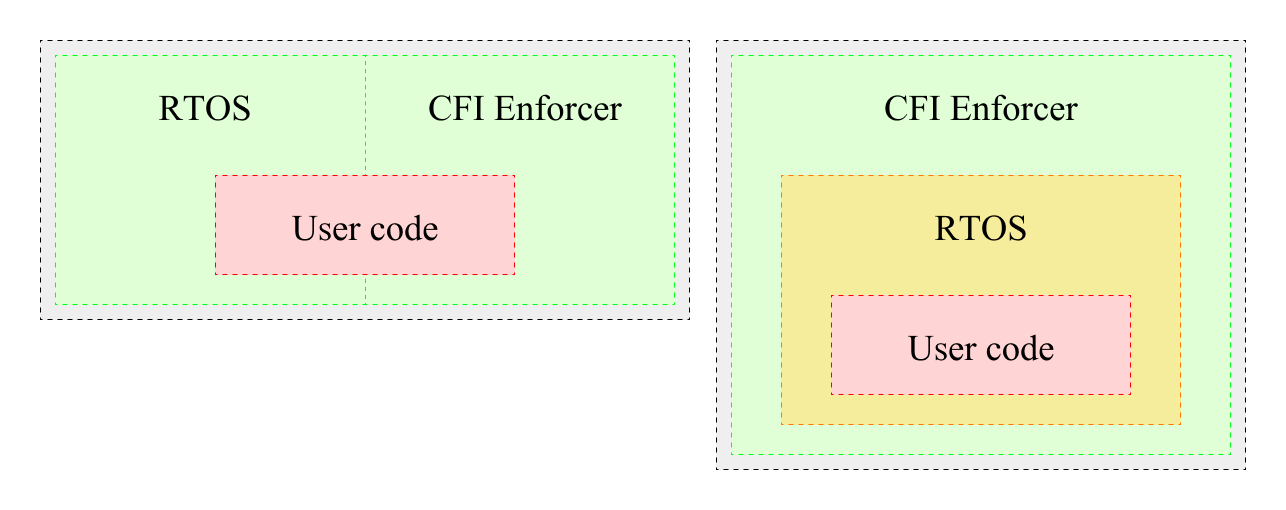
\includegraphics[width=\linewidth]{images/rtos.png}
  \caption{Abstraction of possible RTOS implementations}
  \label{fig:rtos}
\end{figure}

To achieve this result, the first thing we need to do is add the letter \textit{S}
to the Instruction Set Architecture we want to use, making it \textit{RV32IMCS\_ZICSR}
to add supervisor capabilities to our \textit{RISC-V} ISA.

For the second step, we need to import the files required by the RTOS. Since
many RTOSes are designed with a modular approach, not every file is necessary.
For example, we may want to import only the kernel itself, or if we need
networking capabilities, we would need to import the connectivity-related source
files and so on.

Lastly, we need to modify the instrumentation phase in two ways. Firstly, we
need to add, as a target for instrumentation, the source code of the RTOS if we
wish to enforce Control Flow Integrity on it. This can be done by simply adding the
files related to the RTOS to the list \textit{files\_to\_instrument} inside the
\textit{flasher.py} file. Secondly, we need to add the regexes and instrumentation
capabilities to delegate CSR instructions to the interrupt vector table of the project.
This is needed if we want the RTOS to run as supervisor since, from such a privilege
level, it has no access to Control and Status Registers. A solution to this implementation
is deeply discussed in section \ref{sec:rtos_limitations} where we discuss each step
needed to effectively modify the instrumentation phase to address the CSR access
limitation.

In conclusion, to make the building process easier, we may add a simple parameter
to the input of \textit{flasher.py}. As of now, the file can be launched with
the commands described in section \ref{sec:project_instrumentation} but, by simply
adding a parameter like \textit{RTOS=(y/n)}, we could launch \textit{flasher.py}
with \textit{python3 flasher.py command rtos}. Such simple modification would
make it easier to either include the RTOS files or not, thus providing a simple and
fast building process for any kind of project.